\section{Adversarial machine learning}
\label{sec-review}

Adversarial machine learning is concerned with learning a program that is to be robust to adversarial attacks~\cite{aml_book}. The range of possible learning programs and adversarial attacks is broad. For example, we may consider learning a spam detector robust to an adversary that may \textit{attack} the system is such a way that the program detects its spam as non-spam. Alternatively, a program that provides personalized suggestions may have learned sensible information about its users. An adversary may have an incentive to attack the system, such that it has access to this private information. These examples demonstrate the breadth of possible attack vectors that a program may have. Furthermore, as more of our life is digitized, bad actors have increasingly more incentives to attack and jeopardize these systems. This motivates the study of adversarial machine learning and the search for formal guarantees that we can obtain. As such, we will provide a general characterization of adversarial machine learning using a commonly used framework~\cite{aml_book}, followed by a game-theoretic view of the possible equilibrium guarantees that were formulated in the literature.

\subsection{Characterization of adversarial machine learning}
A machine learning program has numerous possible vectors of attack. Knowledge of these attack vectors are relevant for both a practitioner that design a machine learning program or a game-theorist that provides formal guarantees of a system. Examples of attack vectors include:
\paragraph{Data poisoning.} Data poisoning refers to the corrupted data provided by an attacker during the training. For example, in a spam detection program, an attacker may provide spam that they labelled as non-spam. A consequence of such an attack is that the decision boundary may be sub-optimal due to poisoned data.
\paragraph{Exploitation of the structure.} When choosing the model and the objective used to train a program, choices about the structure are necessary made. These choices can almost always be exploited. For example, in a maximal-margin classifier, an attack could leverage less relevant features to force a mis-classification. A practical consequence of this effect is the adversarial perturbation of the data that can yield erroneous classification (e.g. Figure~\ref{fig:adv_class}). In this example, the attacker exploited the fact that deep neural networks are brittle 
\paragraph{Exploitation of prediction error} After training, a program may make classification error. Given access to the learned program, these error may be discovered and then exploited.

\begin{figure}
    \centering
    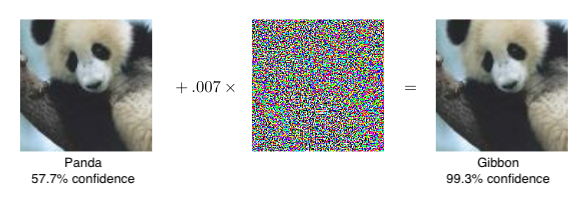
\includegraphics[width=\linewidth]{adversarial_example.png}
    \caption{Example of an adversarial example~\cite{goodfellow_explaining}. The classifier correctly classify the panda (left). But, when adding some random noise (middle), the classifier erroneously classify the panda as a gibbon (right).}
    \label{fig:adv_class}
\end{figure}

More generally, we can qualitatively encapsulate the possible attacks under a taxonomy of attacks against machine learning program. The taxonomy is comprised of three properties: Influence, Security violation and Specificity.
\paragraph{Influence} Describes the capacity of the attacker. The influence can be decomposed into two categories:
\begin{itemize}
    \item \textbf{Causative}: The attacker has the ability to poison the data during training.
    \item \textbf{Exploratory}: The attacker has the ability to exploit the predictions.
\end{itemize}
\paragraph{Security violation} Indicates the type of security violation that an attacker can cause. The security violation is three-fold:
\begin{itemize}
    \item \textbf{Integrity} of the system via false negatives.
    \item \textbf{Availability} of the system and robustness to denial of service.
    \item \textbf{Privacy} and protection of the data used to train the system.
\end{itemize}
\paragraph{Specificity} Refers to how broad the attack is. We define two category:
\begin{itemize}
    \item \textbf{Targeted} refers to attacks that focus on a particular instance.
    \item \textbf{Indiscriminate:} Refers to an attack that broadly affect multiple instances.
\end{itemize}

Now that we have described a framework to view adversarial machine learning, we will see how the problem can be viewed as a game theoretical problem.

\subsection{Game theoretical view of adversarial machine learning}

Now that we have described what is adversarial machine learning, we can see how this problem has been framed as a game theoretic problem. We will assume two players: the learner and the adversary. The role of the adversary is to achieve one of the security violation defined above (e.g. break the integrity/availability of the system or obtain private information). The role of the learner is to perform a task while being robust to an adversary. Formally, we define a learner $f:\mathcal X\to \mathcal Y$ learned by solving an optimization problem similarly to what was defined in Section~\ref{sec:background}. We will write the objective function of the learner $\mathcal{L}_f$ (i.e. the sum of the risk and the regularizers). The adversary is defined as a generative model $g:\mathcal X\to \mathcal X$ which is also learned by solving an optimization problem. We will write the objective function of the adversary $\mathcal{L}_g$. The concrete definition of both the learner and the adversary as well as their objective function depends on the precise problem formulation. 

There are multiple ways to frame and analyze adversarial machine learning. We will first view it as a \textbf{simultaneous game}. Next, we will consider it as a \textbf{Stackelberg game} which is defined as a sequential game where one player is the \textit{leader} (plays first) while the other player is the \textit{follower} (plays second). Finally, we will view how this game can be viewed as a \textbf{Bayesian game}.
\subsubsection{Simulatenous game} 
In a simultaneous game, the two agents play their move at the same time. Although, it finds few practical applications for adversarial machine learning, this setup can be considered theoretically. In general, adversarial machine-learning is typically modeled as a non-cooperative game. That is, the game, represented in normal form, is given by $(N, A, U)$ where $N$ is the set of players, $A$ is the set of actions $A_i$ that a player $i$ can take and $U$ is the set of utilities $U_i$ that each player can have given their action and the actions of the other players. A player's strategy set $S_i=\{\pi(A_i):\pi(A_i)\geq 0~\forall i, \sum_{A_i}\pi(A_i)=1\}$ defines a probability distribution over its action. In this setup, we define a Nash Equilibrium a point where all the players have reached a best response strategy $s_i$ in which they cannot improve their utility further. Formally, a Nash equilibrium is defined as follow \[U(s_i, s_{-i})\geq U(s_i',s_{-i})~\forall i\in N.\]
In our setup, the set of strategy correspond to the action taken by each of our agent defined by the respective parameterized functions $f$ and $g$ for the learner and the adversary respectively. The utility itself can be defined as the inverse of the loss function $\mathcal{L}$. Therefore, an alternative view of a Nash equilibrium in our setup with one adversary and one learner is
\[
\mathcal{L}_f(\mathcal{D},f,g)\leq\mathcal{L}_f(\mathcal{D},f',g) \text{ and } \mathcal{L}_g(\mathcal{D}, f,g)\leq\mathcal{L}_g(\mathcal{D},f,g').
\]
The existence of Nash Equilibrium is not guaranteed in non-cooperative games. can be categorized as zero-sum games or general non-zero sum games. \paragraph{Zero-sum games.} In 2-players zero-sum games, the objective of each player is diametrically opposed. In other words, each player has the same objective, except that one minimizes it, while the other maximizes it. More formally, for our adversarial learning setup,  $\mathcal{L}_f=\mathcal{L}_g=\mathcal L$ and
\[
\max_g\min_f\mathcal{L}(\mathcal{D},f,g) = \min_f\max_g \mathcal{L}(\mathcal{D},f,g).
\]
In zero-sum games, if $f$ and $g$ are linear function, the Nash Equilibrium can be computed using the mini-max theorem. Several work considered this formulation to propose methods to find a Nash equilibrium given different assumptions.

An assumption that may be considered is that the adversarial data lie in a certain confidence interval~\cite{Ghaoui_robust_classification,Lanckriet_robust_minimax}. For example, consider the data points with $\bm x\in\mathbb{R}^d$ and $\bm\sigma\in\mathbb{R}^d$ their interval of confidence. Consider the training set $X$ with $\Sigma$ the intervals for the set of $N$ points, both a $d\times N$ matrix. Finally, consider $\rho$ the sensitivity of the region. Using this object, we can define a hyper-rectangle defining the region where the generator can generate points
\[
\mathcal{X}(\rho) = \{Z\in\mathbb{R}^{n\times N}: X-\rho\Sigma\leq Z\leq X+\rho\Sigma\}.
\]
We assume that the generator is a linear map $g:X\to\mathcal{X}(\rho)$. Assuming that the learner $f$ is also a linear map, the objective function is
\[
\min_f\max_{g:X\to\mathcal{X}(\rho)}\mathcal{L}(X, \Sigma, \bm y, f, g).
\]
$\mathcal{L}$ can be defined as a well defined loss, for example the logistic regression, the Hinge loss, etc. This method render a classifier robust to any perturbation within the trust-region~\cite{Ghaoui_robust_classification}.

Others have considered a generator that corrupts or deletes certain features~\cite{Globerson_robust_deletion,dekel_corrupted_learning}. In the setup where the generator delete certain features, assume that the generator outputs a mask $h:\bm x\to \bm m$ with $m_i\in\{0,1\}~\forall i$. We constraint that $\sum_i m_i = K$ where $K$ is a hyper-parameter. In such a case, the objective of the adversary is corrupt the features in order to maximize the loss and the learner's objective is to be robust to the worst-case corruption. Formally,
\[
\min_f\max_{g:\bm x\to\bm m|\sum_m=K}L(\bm x\odot \bm m, \bm y, f, h).
\]
$\odot$ is defined as the element-wise product. 

\paragraph{Non-zero sum games} However, it can be noted that zero-sum games are overly pessimistic for adversarial machine learning. Intuitively, the objective of the adversary is rarely diametrically opposed to the one of the learner. For example, in a spam detection game, the objective of the adversary is to induce its spam as false-positive. But, the adversary is indifferent to whether the spam detector correctly classify true-positive. The consequence of choosing an objective that is overly pessimistic is that we may incur a learner with inferior performance. For example, a spam detector may be more prone to classify a message as spam and in turn increase the number of false-positive. Therefore, general games are often a better choice to characterize adversarial machine learning games, although PSNE may not always exist and/or may be hard to compute. In any case, a more general formulation has to be considered. We have to consider two potentially different risk for the learner and the adversary that we will denote $\mathcal{R}_f$ and $\mathcal{R}_g$ respectively. We also denote the regularizers for the learner and the adversary $\Omega_f$ and $\Omega_g$ respectively. Their objective functions are \[\mathcal{L}_f=\mathcal{R}_f(\mathcal{D},f,g) + \lambda_f\Omega_f(f)\] and \[\mathcal{L}_g=\mathcal{R}_g(\mathcal{D},f,g)+\lambda_g\Omega_g(\mathcal{D},h)\] for the learner and the adversary respectively. The regularizer for the adversary ensures that it cannot modify the data distribution arbitrarily. An example of such a regularizer is
\[
\Omega_g(\mathcal{D}, g) = \dfrac{1}{n}\sum_{i=1}^n||\bm x_i - g(\bm x_i)||^2.
\]
This more general setup is amenable to games with more than two players. For example, there could exist multiple adversaries. But, without loss of generality, we will keep considering two players, the learner and the adversary, for simplicity. More importantly, it is possible to show the existence and, in some case, the uniqueness of Mixed Nash Equilibrium~\cite{bruckner_static_aml,dritsoula_game_ml}. A Mixed Nash Equilibrium is a set of strategies, i.e. a learner and an adversary sampled from distributions $\pi_f$ and $\pi_g$ respectively, such that
\[
E_{f\sim\pi_f,g\sim\pi_g}\mathcal{L}_f(\mathcal{D},f, g)\leq E_{f' \sim\pi_{f'}, g\sim\pi_g}\mathcal{L}_i(\mathcal{D},f', g),
\]
\[ 
E_{f\sim\pi_f,g\sim\pi_g}\mathcal{L}_f(\mathcal{D},f, g)\leq E_{f \sim\pi_{f}, g'\sim\pi_{g'}}\mathcal{L}_i(\mathcal{D},f, g').
\]


Given the following strong assumption, a unique Mixed Nash Equilibrium exists~\cite{bruckner_static_aml}:
\begin{itemize}
    \item The loss functions $\mathcal{L}_f$ and $\mathcal{L}_g$ are convex and twice continuously differentiable;
    \item The regularizers $\Omega_f$ and $\Omega_g$ and uniformly strongly convex and twice continuously differentiable;
    \item The set of free-parameters of the functions $f$ and $g$ are non-empty, compact, and convex subset of finite-dimensional Euclidean spaces.
\end{itemize}
While being a strong result, these assumptions are restrictive for practical applications. 

A slightly less restrictive and different setup was considered in~\cite{dritsoula_game_ml} in which they prove the existence of Mixed-Strategy Nash Equilibrium. However, they do not show uniqueness of such an equilibrium. In their setup, they consider the case where the learner has to detect the adversary. In this more restricted case, they show existence of a Mixed Nash Equilibrium.

We will now consider non-competitive games in a sequential game framework.

\subsubsection{Stackelberg game} A slightly different framework for describing adversarial machine learning games is Sequential games (i.e. Stackelberg game). In this setup, each player takes turn in selecting their strategy. The first player is called the leader while the second player is called the follower. When taking its action, the follower has knowledge of the leaders strategy profile. While we could theoretically alternate the follower and the leader as in a mouse and cat game~\cite{barreno_security_ml}, we are interested in finding an equilibrium in which both the learner and the follower are stable. Depending on the which player is the leader or the follower, we may have different Stackelberg equilibrium. The case where the leader is the adversary and the follower is the classifier has been considered in some work~\cite{murat_adversarial_classification,liu_game_theoretical_aml}. While interesting, it is not practically realistic for the problem of robustness to adversarial machine learning. We will instead consider the more realistic case where the leader is the classifier and the follower is the adversary~\cite{bruckner_stackelberg}. We will also assume that the follower (i.e. the adversary) will play rationally according to its objective function and that the learner has knowledge about the objective function of the adversary. For example, a learner classifying spams would know that the objective of the adversary is to maximize the number of spams.

More formally, we assume that the adversary is learning a transformation $g$ given an optimal $f'$
\begin{equation}
\label{eqn-stackle_gen}
    \min_g \mathcal{L}_g(\mathcal{D}, f', g).
\end{equation}
This amount to solving a regular optimization problem because $f'$ is known at the time of the optimization.

Assuming that the adversary will solve the above optimization problem to choose its $g'$, the learner choose the model $f$ that minimizes its objective function $\mathcal{L}_f$.
\[
\min_f \mathcal{L}_f(\mathcal{D}, f, g'),
\]
Further, the optimal $g'$ might not be unique. In fact, a set $g'\in\mathcal{G}'$ might solve Equation~\eqref{eqn-stackle_gen}. In this case, two view may be possible: the optimist and the pessimist view. For example, if we assume the worst case when learning the model $f$, we may solve the following optimization problem:
\[
\min_f\max_{g'\in\mathcal{G}'} \mathcal{L}_f(\mathcal{D}, f, g').
\]
A Stackleberg equilibrium can be identified by backward induction: the learner chooses $f'$ that maximizes its utility with respect to the attacker’s response g'. More specifically, the equilibrium can be found by solving the following bilevel optimization problem where the objective of the learner is the outer loop and the objective of the adversary is the inner loop. Assuming a unique $g'$:
\begin{equation}
    \label{eqn-bilevel}
    \begin{split}
        &\min_f \mathcal{L}_f(\mathcal{D}, f, g')\\
        & \text{ s.t. } g' = \arg\min_{g}\mathcal{L}_g(\mathcal{D}, f, g).
    \end{split}
\end{equation}
Bilevel optimization are NP-hard to solve exactly, even in cases where the objectives are linear~\cite{jeroslow_polynomial_bilevel}. Different method exists to relax the problem, such as relying on greedy search method like gradient descent~\cite{naveiro_gradient_stackelberg} or adding regularizers, at the cost of losing the optimality guarentees~\cite{colson_bilevel}.

It is possible to solve the above problem by constraint further the problem and considering a special case of the bilevel optimization. Assume that the regularizers $\Omega_f$ and $\Omega_g$ are strongly convex that the risk of the adversary $\mathcal{R}_g$ is convex and that $f:X\to\mathbb{R}$ is linear. Further, assume that the inner optimization problem is replaced with its Karush-Kuhn-Tucker conditions. We can do so by considering a set constraints $\bm\tau$ defined in the inner optimization problem of the optimization problem as shown in the following optimization problem
\begin{equation}
    \label{eqn-convex-stack}
    \begin{split}
    &\min_{f_\theta}, \dfrac{1}{n}\sum_{i=1}^n\mathcal{R}_f(f_\theta(x_i) + \tau_i||\theta||^2, y_i) + \dfrac{\lambda_f}{2}||\theta||^2\\
    &\text{ s.t. } \forall~i: 0=\tau_i + \dfrac{n}{\lambda_g}\mathcal{R}_g(f_\theta(x_i) + \tau_i||\theta||^2, y_i).
    \end{split}
\end{equation}
The Stackelberg prediction game from Equation~\eqref{eqn-convex-stack} attains an equilibrium where $g':\bm x_i\to \bm x_ + \tau_i\bm w$~\cite{bruckner_stackelberg}. The solution to this problem can be obtained by a sequential quadratic programming method. 

While this analytic formulation is very contrived, it is possible to use numerical approaches to approximate a solution. One way to approximate Equation~\eqref{eqn-bilevel} is by following a PDE-constrained optimization problem~\cite{naveiro_gradient_stackelberg}. Assume $f$ and $g$ linear, and that the inner problem of Equation~\eqref{eqn-bilevel} has a unique solution $g'$ for each $f$. We define the following differential equation $G:f\times t\to g$, where $t\in\mathbb{R}_+$ is a time variable. In can be shown under mild condition that the following constrained optimization problem converges with $G(f,t)\to g'$ as $t\to\infty$ with rate $\mathcal O(\dfrac{1}{t})$~\cite{naveiro_gradient_stackelberg}:
\begin{equation*}
    \begin{split}
        &\min_f \mathcal{L}_f(\mathcal{D}, f, G(f,T))\\
        \text{ s.t. } &\partial_tG(f, t) = \partial_G\mathcal{L}_g(\mathcal{D}, f, G(f, t))\\
        & G(f, 0) = 0.
    \end{split}
\end{equation*}


\subsubsection{Bayesian game}
So far, we assumed that each player had the knowledge about the other's player objective function. However, in practice, such an assumption may be hard to meet. For example, we may  not know that the objective of the adversary is to send spam related to a particular product, for example car insurances. In such a case, we want to relax the assumption that both players has knowledge about the other's objective and consider non-cooperative games with incomplete information. In this case, the uncertainty over the objective function of the other player is modeled using the Bayesian framework. This framework is usually referred as the Bayesian game~\cite{harsanyi_bayesian_games}.

In the Bayesian game, we can assume that the cost $c$ is a random variable following some prior $q(c)$. For example, assume a learner that have incomplete information about the cost $c_a$ of the adversary. We can further assume that $g=\mathcal{G}(c_a)$ is not a function of $c_a$ for all practical purpose. We can now define an objective function that consider the uncertainty:
\begin{equation}
\label{eqn-bayesian_learner}
    \min_f\int_{c_a}\mathcal{L}_f(\mathcal{D}, \mathcal{G}(c_a), f)dq(c_a).
\end{equation}
Assuming that the adversary have knowledge of the learners objective, we can define its objective
\begin{equation}
    \label{eqn-bayesian_adverary}
    \min_g\mathcal{L}_g(\mathcal{D}, f, g).
\end{equation}
We define a Bayesian Equilibrium a $f$ and $\mathcal{G}(c_a)$ that satisfy Equation~\eqref{eqn-bayesian_learner} and Equation~\eqref{eqn-bayesian_adverary}~\cite{harsanyi_bayesian_games}. If $q$ is a Dirac distribution, we recover a Nash Equilibrium. We can now ask the usual question as to whether such an equilibrium may exists? Under which condition it exists? If fact, it can be shown that such an equilibrium exists if $f$ and $g$ are compact and convex~\cite{groshan_bayesian_reg}.

The above results is concerned with Simultaneous Bayesian games. But what can we say about Stackelberg Bayesian games? Unsurprisingly, it is NP-hard in the general case for both Pure Nash Equilibrium and Mixed Nash Equilibrium~\cite{conitzer_bayesian_game}. 
